\chapter{Prototipação}

A prototipação de aplicativos móveis representa uma etapa fundamental no processo de desenvolvimento de software, constituindo-se como uma metodologia essencial para validação de conceitos, refinamento de funcionalidades e otimização da experiência do usuário antes da implementação final. Segundo estudos recentes, a experiência do usuário, interação usuário-produto e produtos digitais tornaram-se tópicos cada vez mais populares nas disciplinas de design nos últimos anos, evidenciando a crescente importância da prototipação no desenvolvimento de aplicações móveis \cite{sciencedirect_design_approaches}.

Definida como o processo de criação de versões preliminares e funcionais de uma aplicação, a prototipação permite aos desenvolvedores e designers testarem hipóteses, identificarem problemas de usabilidade e validarem soluções antes do investimento em desenvolvimento completo. A prototipação de aplicativos móveis é essencial para agilizar o desenvolvimento, melhorar a experiência do usuário e reduzir redesigns custosos \cite{decode_benefits}.

\section{Finalidades e Benefícios}

A prototipação de aplicativos móveis serve a múltiplos propósitos estratégicos no ciclo de desenvolvimento de software. Primeiramente, funciona como uma ferramenta de validação de conceitos, permitindo que equipes testem ideias e funcionalidades de forma iterativa e com baixo custo. Os protótipos de aplicativos móveis são poderosos e benéficos, oferecendo vantagens significativas em termos de economia de recursos e otimização de resultados \cite{gojilabs_essential}.

Entre os principais benefícios identificados na literatura, destaca-se a redução significativa de riscos de projeto. A prototipação oferece insights para refinar ainda mais a aplicação, sendo uma fase importante no desenvolvimento de aplicativos móveis \cite{softsuave_guide}. Adicionalmente, o processo facilita a comunicação entre stakeholders, permitindo visualização concreta de ideias abstratas e alinhamento de expectativas \cite{okoone_benefits}.

Atualmente, mais de 5,2 bilhões de dispositivos móveis únicos estão ativos mundialmente, destacando a escala massiva e o alcance da tecnologia móvel \cite{netguru_prototyping}. Este contexto reforça a importância estratégica da prototipação, considerando que dispositivos móveis representam 54\% de todo o tráfego web global, indicando uma mudança em direção a padrões de consumo mobile-first \cite{netguru_prototyping}.


\section{Aplicações Contemporâneas}

O campo da prototipação de aplicativos móveis tem evoluído significativamente com a incorporação de tecnologias emergentes. O mercado de aplicativos móveis é caracterizado por um grande número de aplicações frequentemente desenvolvidas por empresas menores, o que torna a prototipação ainda mais crucial para validação de viabilidade antes do investimento em desenvolvimento completo \cite{researchgate_ai_prototyping}.

Estudos recentes demonstram aplicações inovadoras da prototipação, incluindo o desenvolvimento de protótipos de aplicativos móveis focados na melhoria do aprendizado na área de matemática, utilizando metodologia Design Sprint para determinar características de usabilidade e aceitação por estudantes \cite{salud_ciencia_prototyping}. Estas aplicações evidenciam o potencial da prototipação não apenas como ferramenta de desenvolvimento, mas também como instrumento de pesquisa e inovação educacional.

\section{Considerações Metodológicas}

A implementação efetiva da prototipação requer consideração cuidadosa de aspectos metodológicos e ferramentais. Aprender a dominar a prototipação de aplicativos móveis pode economizar custos, melhorar a satisfação do usuário e agilizar o processo de desenvolvimento através de ferramentas efetivas \cite{decode_best_practices}.

A execução de protótipos pode fornecer insights para refinar ainda mais a aplicação, sendo fundamental seguir melhores práticas estabelecidas na literatura para maximizar os benefícios do processo \cite{ossisto_guide}. A seleção adequada de ferramentas e metodologias deve considerar fatores como complexidade do projeto, recursos disponíveis e objetivos específicos de validação.


\section{Protótipo SheSafe}

\subsection{Protótipo inicial}
\begin{figure}[h]
	\begin{center}
		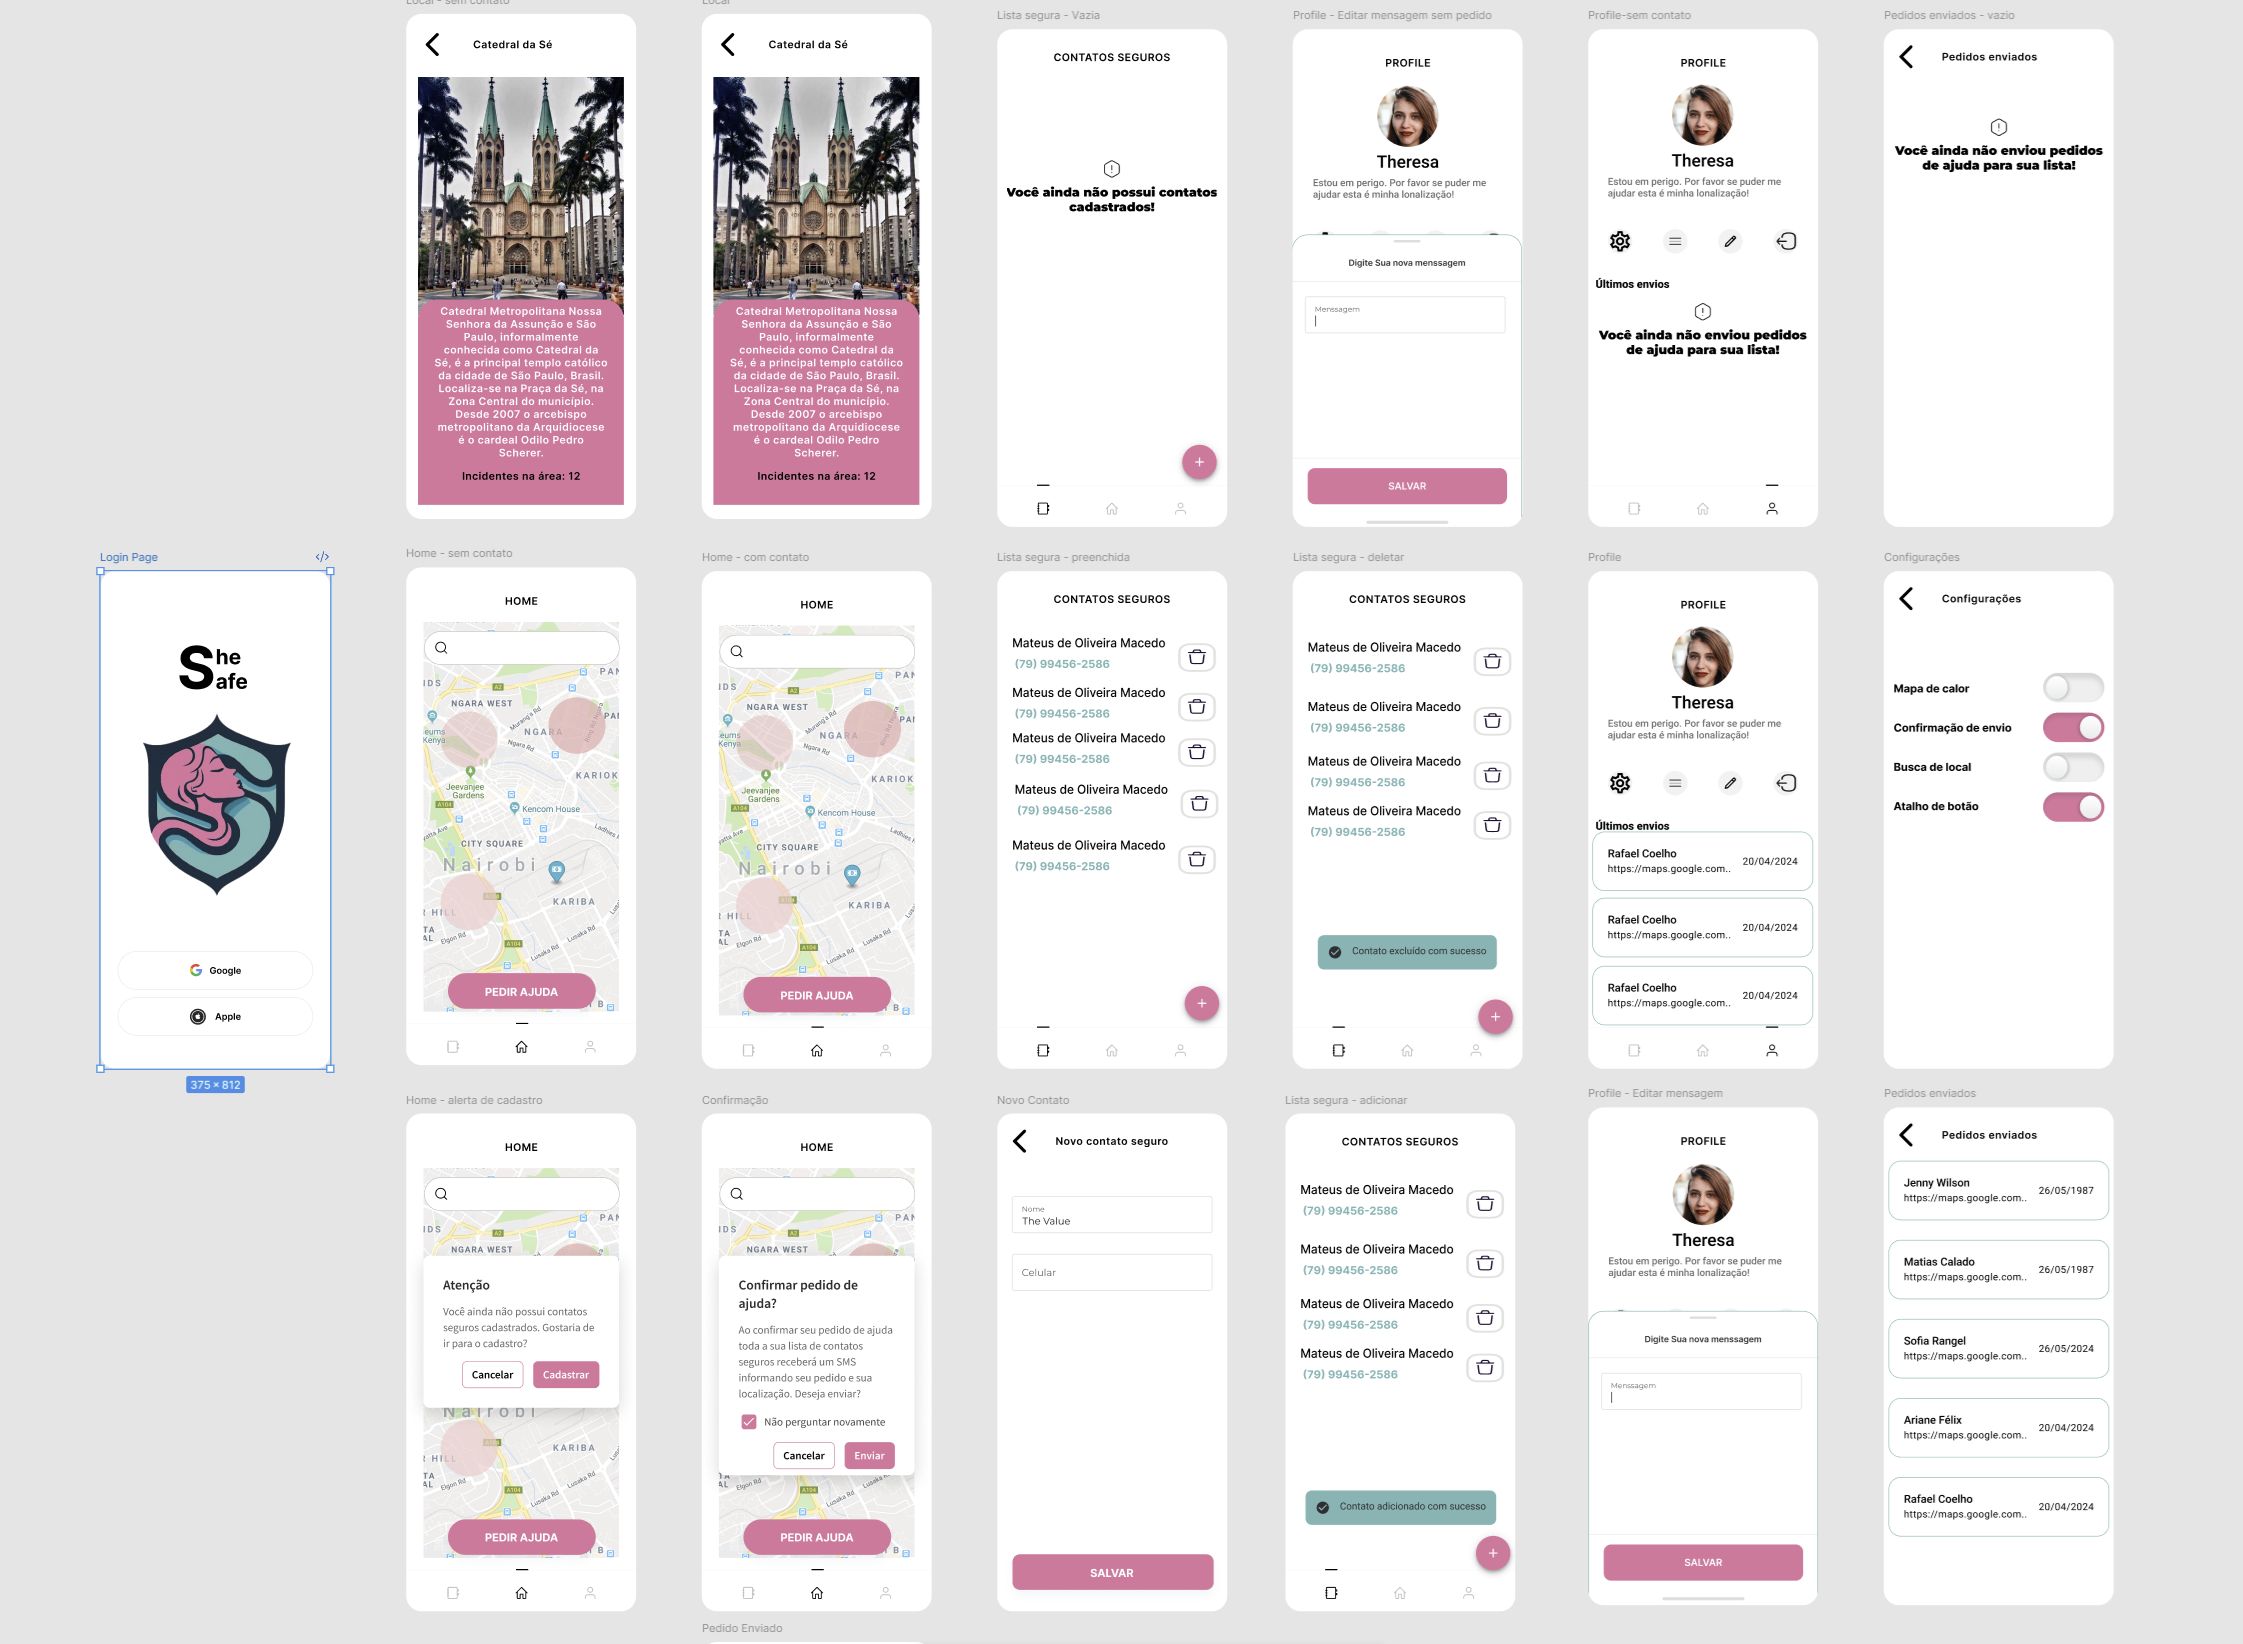
\includegraphics[width=0.8\linewidth]{images/prototipo-inicial.png}\\
	\end{center}
	\caption[Pr]{Protótipo inicial}
	\label{fig:prototipo-inicial}
	\legend{Fonte: Próprio Autor}
\end{figure}
\pagebreak

O protótipo inicial pode acessado através do link: \href{https://www.figma.com/proto/ZOxt5eHuQt0RjhagaDpuXU/SheSafe?type=design&node-id=26-369&viewport=1892%2C1064%2C0.71&t=gZiNpzVt2mGhuMDV-0&scaling=min-zoom&starting-point-node-id=26%3A653}{SheSafe - Protótipo Inicial}

\subsection{Protótipo final}
\begin{figure}[h]
	\begin{center}
		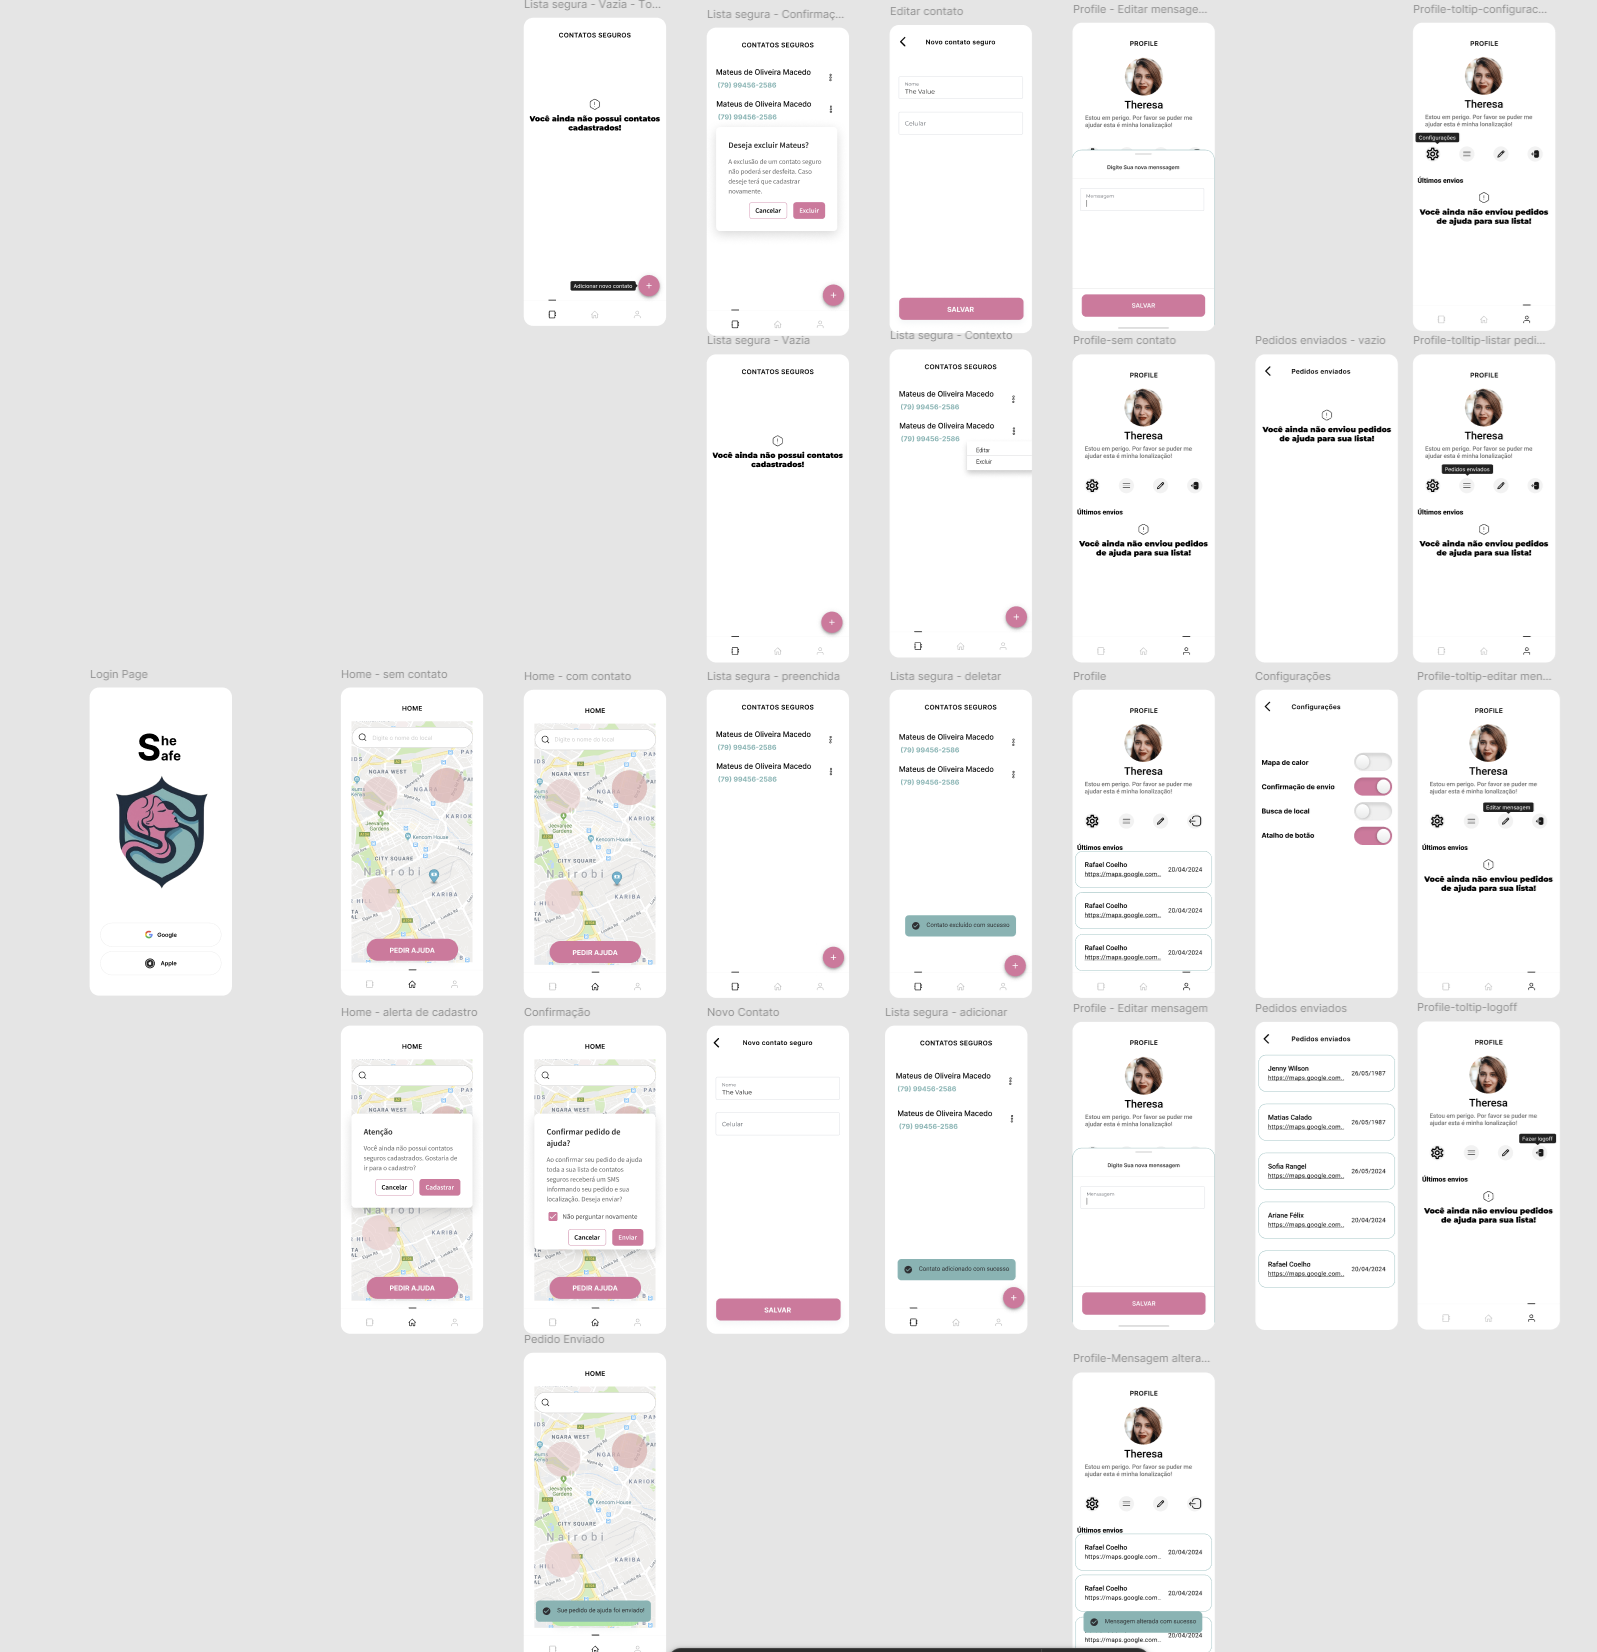
\includegraphics[width=0.7\linewidth]{images/prototipo-final.png}\\
	\end{center}
	\caption[Pr]{Protótipo final}
	\label{fig:prototipo-final}
	\legend{Fonte: Próprio Autor}
\end{figure}
\pagebreak
O protótipo final pode acessado através do link: \href{https://www.figma.com/proto/GALwTZKTsmvOVWX4JARmOB/SheSafe-Corrigido?node-id=26-653&viewport=2654%2C786%2C0.79&t=dkVCQTw83BbPw3KK-0&scaling=min-zoom&starting-point-node-id=26%3A653}{SheSafe - Protótipo Final}

Foi realizada uma cópia do projeto inicial para realizar as melhorias e alterações propostas pelas avaliações rasteira, heurística e de usabilidade.

\section{Melhorias Aplicadas}
Foram realizadas algumas mudanças no protótipo inicial até chegar no produto final. Tais melhorias foram realizadas com base nas avaliações aplicadas a público externo. Dentre elas estão:

\begin{itemize}
\item Tela 7 – alteração do título da tela para atender a corretamente ao que se propõe.
\item Tela de lista de contato – foi adicionado um menu de contexto com a opções de editar e excluir contato atendendo ao apontamento de não ser possível editar o contato.
\item Tela de listagem de contato – foi adicionado um dialog de confirmação de exclusão para atender ao apontamento de prevenção de exclusão acidental.
\item Tela 6 – foi alterado o ícone do menu de logoff para melhor exibir a intenção do menu.
\item Tela de alteração de mensagem – foi adicionada um feedback informando o sucesso da alteração da mensagem padrão do pedido de ajuda.
\item Campo de busca – adicionado hint explicativo para atender ao apontamento de não saber o que inserir no campo se busca.
\item Ícone de voltar – aplicada a redução do padrão de tamanho do ícone de voltar para atender ao apontamento recebido.
\item Botão de adicionar contato – foi introduzido um click longo para exibir um toltip explicando o que a ação do botão faz.
\item Menu de ações tela 6 – foi adicionado um toltip para ação de pressionar e segurar para os menus de ações da tela 6 atendendo ao apontamento de não saber exatamente o que cada menu faz. Com o toltip o menu passa a ter uma mensagem de contexto informado o que sua ação está encarregada.
\item Card de pedido enviado – aplicado estilo sublinhado no link do maps que contêm a localização do usuário atendendo ao apontamento sobre não reconhecer como link na tela o texto.
\item Dialogs – aplicado um pouco mais de peso no fundo dos botões de ação que ficam internos dentro dos dialogs para um melhor contraste.

\end{itemize}